\documentclass[tikz,border=10pt]{standalone}
\usepackage{amsmath}
\usetikzlibrary{calc}

\begin{document}
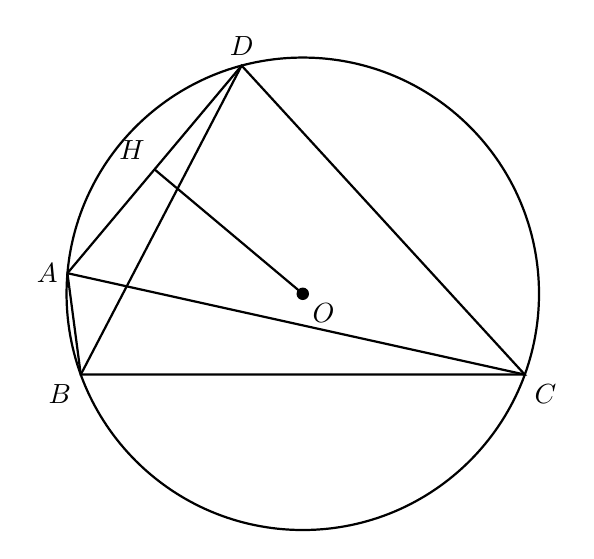
\begin{tikzpicture}[>=stealth, scale=1.5]
    % 定义各点坐标，运用精确角度确保 AC 垂直 BD
    \coordinate (O) at (0,0);
    \coordinate (A) at (175:2);
    \coordinate (B) at (200:2);
    \coordinate (C) at (-20:2);
    \coordinate (D) at (105:2);
    
    % 修正 H 点：使用 calc 插件直接计算 A 和 D 的中点，确保其必在线段 AD 上
    \coordinate (H) at ($(A)!0.5!(D)$);

    % 绘制外接圆
    \draw[thick] (O) circle (2);

    % 绘制多边形和对角线
    \draw[thick] (A) -- (B) -- (C) -- (D) -- cycle;
    \draw[thick] (A) -- (C);
    \draw[thick] (B) -- (D);
    
    % 绘制从圆心到中点的垂线 OH
    \draw[thick] (O) -- (H);

    % 标注圆心点和各字母
    \fill (O) circle (1.5pt) node[below right] {$O$};
    \node[left] at (A) {$A$};
    \node[below left] at (B) {$B$};
    \node[below right] at (C) {$C$};
    \node[above] at (D) {$D$};
    \node[above left] at (H) {$H$};
\end{tikzpicture}
\end{document}